% arara: pdflatex
% arara: convert: {density: 160, otheroptions: -dispose previous -delay 10 -loop 1, format: gif}
% arara: showfile: {format: gif}
\documentclass{beamer}

\usetheme{Madrid}

\usepackage{tikzducks}
\usetikzlibrary{positioning}
\newcommand{\ducky}[3]{\begin{scope}[shift={(#1,#2)}, scale=.3]
		\duck[body=#3]
\end{scope}}

\begin{document}
\begin{frame}
\frametitle{Christmas Ducks 1}
	\centering
	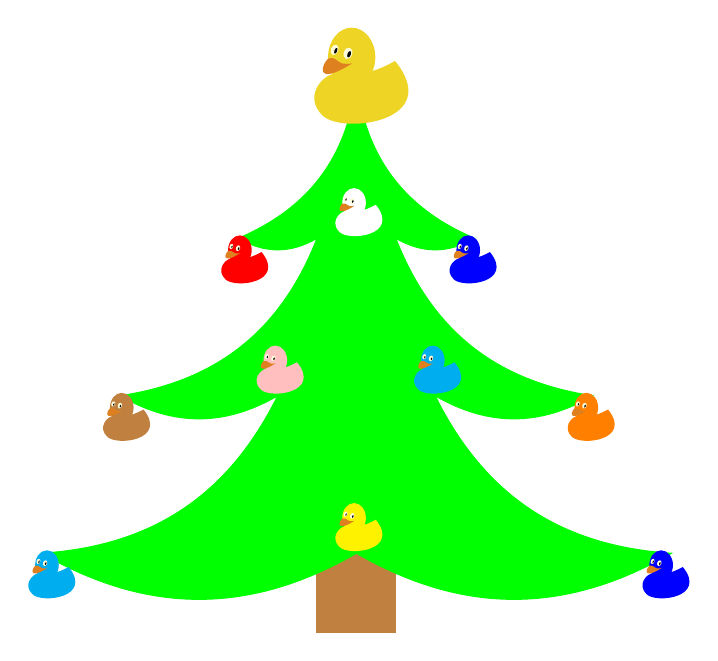
\begin{tikzpicture}
	\filldraw[brown] (-.5,0) rectangle (.5,1); 
	\filldraw[green] (0,1) 
	to[bend right] ++(4,0)
	to[bend left] ++(-3,2)
	to[bend right] ++(2,0)
	to[bend left] ++(-2.5,2)
	to[bend right] ++(1,0)
	to[bend left] ++(-1.5,2)
	-- cycle;
	\filldraw[green] (0,1) 
	to[bend left] ++(-4,0)
	to[bend right] ++(3,2)
	to[bend left] ++(-2,0)
	to[bend right] ++(2.5,2)
	to[bend left] ++(-1,0)
	to[bend right] ++(1.5,2)
	-- cycle;
	\begin{scope}[shift={(-.6,6.4)}, scale=.6]
	\duck
	\end{scope}
	\ducky{-1.75}{4.4}{red}
	\ducky{1.15}{4.4}{blue}
	\ducky{-3.25}{2.4}{brown}
	\ducky{2.65}{2.4}{orange}
	\ducky{-4.2}{.4}{cyan}
	\ducky{3.6}{.4}{blue}
	\ducky{-.3}{5}{white}
	\ducky{-1.3}{3}{pink}
	\ducky{.7}{3}{cyan}
	\ducky{-.3}{1}{yellow}
	\end{tikzpicture}
\end{frame}
\begin{frame}
	\frametitle{Christmas Ducks 2}
	\centering
	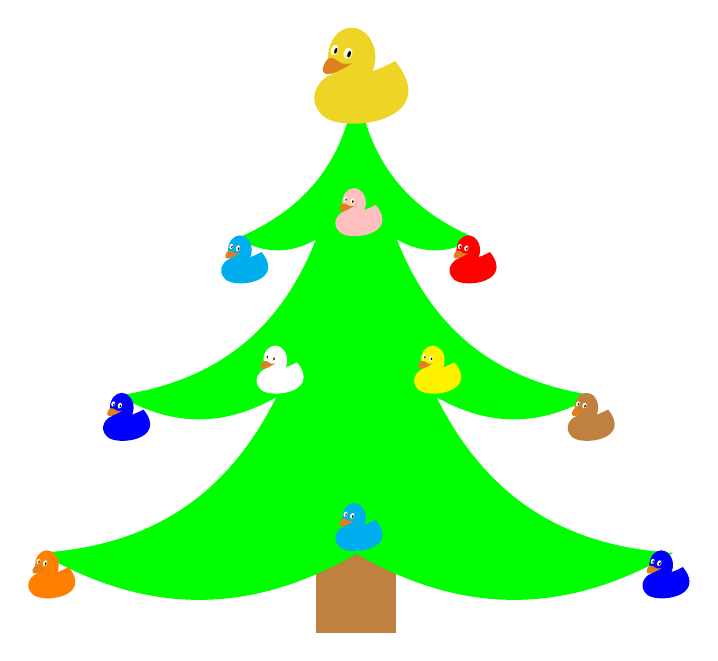
\begin{tikzpicture}
	\filldraw[brown] (-.5,0) rectangle (.5,1); 
	\filldraw[green] (0,1) 
	to[bend right] ++(4,0)
	to[bend left] ++(-3,2)
	to[bend right] ++(2,0)
	to[bend left] ++(-2.5,2)
	to[bend right] ++(1,0)
	to[bend left] ++(-1.5,2)
	-- cycle;
	\filldraw[green] (0,1) 
	to[bend left] ++(-4,0)
	to[bend right] ++(3,2)
	to[bend left] ++(-2,0)
	to[bend right] ++(2.5,2)
	to[bend left] ++(-1,0)
	to[bend right] ++(1.5,2)
	-- cycle;
	\begin{scope}[shift={(-.6,6.4)}, scale=.6]
	\duck
	\end{scope}
	\ducky{-1.75}{4.4}{cyan}
	\ducky{1.15}{4.4}{red}
	\ducky{-3.25}{2.4}{blue}
	\ducky{2.65}{2.4}{brown}
	\ducky{-4.2}{.4}{orange}
	\ducky{3.6}{.4}{blue}
	\ducky{-.3}{5}{pink}
	\ducky{-1.3}{3}{white}
	\ducky{.7}{3}{yellow}
	\ducky{-.3}{1}{cyan}
	\end{tikzpicture}
\end{frame}	
\begin{frame}
	\frametitle{Christmas Ducks 3}
	\centering
	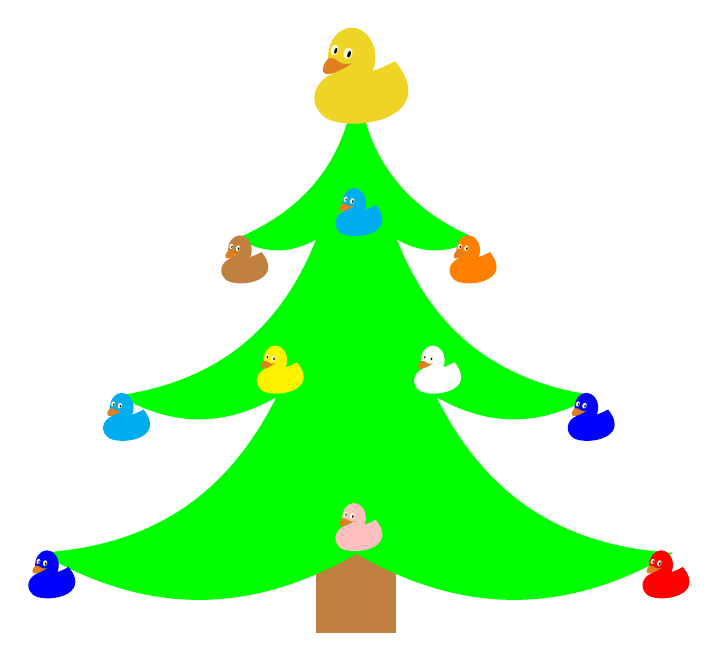
\begin{tikzpicture}
	\filldraw[brown] (-.5,0) rectangle (.5,1); 
	\filldraw[green] (0,1) 
	to[bend right] ++(4,0)
	to[bend left] ++(-3,2)
	to[bend right] ++(2,0)
	to[bend left] ++(-2.5,2)
	to[bend right] ++(1,0)
	to[bend left] ++(-1.5,2)
	-- cycle;
	\filldraw[green] (0,1) 
	to[bend left] ++(-4,0)
	to[bend right] ++(3,2)
	to[bend left] ++(-2,0)
	to[bend right] ++(2.5,2)
	to[bend left] ++(-1,0)
	to[bend right] ++(1.5,2)
	-- cycle;
	\begin{scope}[shift={(-.6,6.4)}, scale=.6]
	\duck
	\end{scope}
	\ducky{-1.75}{4.4}{brown}
	\ducky{1.15}{4.4}{orange}
	\ducky{-3.25}{2.4}{cyan}
	\ducky{2.65}{2.4}{blue}
	\ducky{-4.2}{.4}{blue}
	\ducky{3.6}{.4}{red}
	\ducky{-.3}{5}{cyan}
	\ducky{-1.3}{3}{yellow}
	\ducky{.7}{3}{white}
	\ducky{-.3}{1}{pink}
	\end{tikzpicture}
\end{frame}	
\end{document}